\section{Milestone M2: error mitigation}
\label{sec:m2}

\begin{tcolorbox}[colback=gray!5, colframe=gray!40, title={M2 at a glance}, fonttitle=\bfseries]
  \textbf{Question.} How much of the noise bias can mitigation remove?\quad
  \textbf{Answer so far.} On \py{FakeGuadalupeV2}, readout correction plus total-spin symmetry
  filtering appeared to bring the HVA bias at the exact parameters from \VMtHvaZeroRawRel{} to
  \VMtHvaZeroRoSymRel{} at no extra shots per energy. This report found that the small residual
  is an over-correction of \VMxOverPct{} cancelling the residual noise (\cref{sec:m2cancel}); treating readout consistently
  leaves \VMxHvaZeroFullCtfRel.\\
  \textbf{Code.} Commit \texttt{c9272e3}; results recorded in \texttt{e87051a}; estimator
  corrected in \texttt{56aadd3}. \textbf{Results.} \py{results/m2-evaluation-0},
  \py{results/m2-evaluation-0p3}, \py{results/m2_vqe-summary}. \textbf{Status.}
  \emph{Reopened}: the chosen stack is withdrawn and reruns are in progress; H1 skipped.
\end{tcolorbox}

\subsection{Goal and exit criteria}

After M0 the noisy energy is an honest estimate, but it sits \VMtHvaZeroRawRel{} above the truth at
the exact parameters (\cref{sec:noise}). An optimiser cannot remove that bias
(\cref{prop:mixed}); mitigation can try. M2 implemented four techniques as composable estimator
layers, measured each combination at \emph{fixed} parameters where the noise-free energy is
known, and chose a stack for full optimisations and later hardware runs. Exit: a measured bias
and shot cost for every stack, and a chosen stack.

\subsection{Theory}

All four techniques act on the energy estimator, not on the circuit's parameters. Two of them
need the individual shots, so they replace the Estimator primitive with a sampler that measures
the \VMeasGroups{} bases itself. Since every term of $H$ is $X_iX_j$, $Y_iY_j$ or $Z_iZ_j$, the
three qubit-wise commuting groups are the uniform bases: all qubits measured in $X$, all in $Y$,
or all in $Z$.

\begin{ntn}
  For one basis, a shot is a bit string $b\in\{0,1\}^{n}$, $n=\VNumSites$, and the noise-free
  outcome distribution is $p(b)$. Qubit $q$'s readout flips $0\to1$ with probability $e_0^{(q)}$
  and $1\to0$ with probability $e_1^{(q)}$, independently of the other qubits; its confusion
  matrix is
  $A_q=\bigl(\begin{smallmatrix}1-e_0^{(q)} & e_1^{(q)}\\ e_0^{(q)} & 1-e_1^{(q)}\end{smallmatrix}\bigr)$,
  with columns indexed by the prepared bit and rows by the read bit. A Pauli term $P_t$ of the
  measured basis acts on the support $S_t$, and $s(b)=(-1)^{b}$ is the eigenvalue of bit $b$.
\end{ntn}

\begin{dfn}[Counts-level energy estimator]\label{dfn:counts}
  Given weights $w_q\colon\{0,1\}\to\RR$, a shot $b$ contributes
  $\varepsilon(b)=\sum_t c_t\prod_{q\in S_t}w_q(b_q)$ and the energy estimate is the mean of
  $\varepsilon$ over the shots, summed over the three bases. Without readout correction
  $w_q=s$. With readout correction $w_q=v_q$, where $v_q=(1,-1)\,A_q^{-1}$, that is
  \[
    v_q(0)=\frac{1-e_1^{(q)}+e_0^{(q)}}{1-e_0^{(q)}-e_1^{(q)}},\qquad
    v_q(1)=-\frac{1+e_1^{(q)}-e_0^{(q)}}{1-e_0^{(q)}-e_1^{(q)}} .
  \]
  \emph{Symmetry filtering} discards every shot whose Hamming weight $|b|$ differs from $n/2$
  before the mean is taken.
\end{dfn}

Because $\varepsilon$ is computed per shot, the standard error of the mean is the exact one,
$\operatorname{std}(\varepsilon)/\sqrt{\text{shots}}$, instead of the primitive's upper bound
of \cref{rem:stdbound}.

\begin{prop}[Readout correction is unbiased]\label{prop:readout}
  If the readout errors are independent with confusion matrices $A_q$ and the $v_q$ use the same
  $A_q$, then for every Pauli term $\mathbb E\bigl[\prod_{q\in S_t}v_q(\tilde b_q)\bigr]=\langle P_t\rangle$,
  where $\tilde b$ is the read string and $\langle P_t\rangle$ the noise-free expectation.
\end{prop}

\begin{proof}
  Condition on the prepared string $b$. The read bits are independent with
  $\Pr(\tilde b_q=r\mid b_q)=(A_q)_{r b_q}$, so
  $\mathbb E[v_q(\tilde b_q)\mid b_q]=\sum_r v_q(r)(A_q)_{r b_q}=\bigl((1,-1)A_q^{-1}A_q\bigr)_{b_q}=s(b_q)$.
  Independence turns the expectation of the product over $S_t$ into the product of these
  conditional means, $\prod_{q\in S_t}s(b_q)$, which is the eigenvalue of $P_t$ on $b$. Averaging
  over $b\sim p$ gives $\langle P_t\rangle$.
\end{proof}

The price is variance: $|v_q|\approx1/(1-2e)$, so each two-body term's per-shot magnitude grows
by about $1/(1-2e)^2$. With the calibrated mean flip probability $e=\VMtReadoutErr$ (largest
\VMtReadoutErrMax) this is under $10\,\%$.

\begin{prop}[Ring-ansatz states lie in the zero-magnetisation sector of every basis]\label{prop:sector}
  For every parameter value, the RVB and HVA states $\ket{\psi(\theta)}$ of \cref{dfn:ansatz}
  are total-spin singlets, $\vec S_{\mathrm{tot}}^{\,2}\ket{\psi(\theta)}=0$ with
  $\vec S_{\mathrm{tot}}=\sum_i\vec\sigma_i/2$. Consequently, in each uniform basis $X$, $Y$ or
  $Z$, a noise-free shot has exactly $n/2$ ones.
\end{prop}

\begin{proof}
  The initial state is a product of singlets (\cref{dfn:singlet}), each with total spin $0$, so
  the product has $\vec S_{\mathrm{tot}}^{\,2}=0$. Every later gate is generated by
  $\SWAP_{ij}=\tfrac12(I+X_iX_j+Y_iY_j+Z_iZ_j)$ or by $h_{ij}$, both functions of
  $\vec\sigma_i\cdot\vec\sigma_j$, which commutes with every component of $\vec S_{\mathrm{tot}}$.
  Hence each gate commutes with $\vec S_{\mathrm{tot}}^{\,2}$ and the state stays a singlet.
  Now $0=\bra\psi\vec S_{\mathrm{tot}}^{\,2}\ket\psi=\sum_{\alpha}\lVert S^\alpha_{\mathrm{tot}}\ket\psi\rVert^2$,
  so $S^\alpha_{\mathrm{tot}}\ket\psi=0$ for $\alpha=x,y,z$. Measuring every qubit in basis
  $\alpha$ measures the $\sigma^\alpha_i$, and $S^\alpha_{\mathrm{tot}}=\tfrac12(n-2|b|)$ on outcome
  $b$; only $|b|=n/2$ has nonzero amplitude.
\end{proof}

A shot of any other weight was corrupted by noise and can be discarded \parencite{bonetmonroig2018,mcardle2019}.
This is not free: the filter keeps only about \VMtKept{} of the shots under full device noise,
so the shot noise per energy grows by about $\sqrt2$. It also only detects errors that change
the weight; an error that maps the state to another weight-$n/2$ string passes.

\begin{dfn}[Zero-noise extrapolation by local folding]\label{dfn:zne}
  For an odd scale $\lambda=2k+1$, replace every two-qubit gate $G$ of the transpiled circuit by
  $G(G^\dagger G)^k$ \parencite{giurgicatiron2020}. The unitary is unchanged and the two-qubit
  error is amplified roughly $\lambda$-fold. Measure $E(\lambda)$ at $\lambda=1,3,5$ and fit
  $E(\lambda)=A\,e^{-b\lambda}$ \parencite{endo2018}; report $A=E(0)$.
\end{dfn}

The exponential model is the one suggested by \cref{prop:depol}: if each folded gate multiplied
the energy by a fixed factor, $E(\lambda)$ would decay geometrically in $\lambda$. ZNE triples
the shots per energy.

\begin{dfn}[Twin-circuit rescaling]\label{dfn:twin}
  Choose \emph{twin} parameters $\theta_{\mathrm{t}}$ whose noise-free energy
  $E_{\mathrm{ideal}}(\theta_{\mathrm{t}})$ is computable classically, measure the twin once with
  noise, and report $E_{\mathrm{mit}}(\theta)=E_{\mathrm{noisy}}(\theta)\,
  E_{\mathrm{ideal}}(\theta_{\mathrm{t}})/E_{\mathrm{noisy}}(\theta_{\mathrm{t}})$
  \parencite{urbanek2021}. The package picks the twin on a grid of multiples of $\pi/4$ with the
  largest $|E_{\mathrm{ideal}}|$, excluding ground states so the test is not circular.
\end{dfn}

\begin{rem}[When rescaling is exact]
  Under global depolarising noise of the same strength for both circuits, \cref{prop:depol} gives
  $E_{\mathrm{noisy}}=(1-p)E_{\mathrm{ideal}}$ for target and twin alike, and the ratio cancels
  $(1-p)$ exactly. Rescaling therefore works to the extent that the damping factor
  $E_{\mathrm{noisy}}/E_{\mathrm{ideal}}$ is the same for the twin and the target. Nothing
  guarantees that for real noise, which is neither global nor state-independent.
\end{rem}

\subsection{Implementation}

\begin{itemize}
  \item \textbf{Counts layer} (\py{CountsEnergy} in \py{mitigation/counts.py}): measures the three
    bases itself, with Qiskit's backend sampler over Aer (fresh seed per call, as in M0) or the runtime
    \py{SamplerV2}. Readout is calibrated once per estimator by preparing all-zeros and all-ones
    (2 circuits of 16384 shots). In \texttt{c9272e3}, which produced every result in this chapter,
    shots are \emph{filtered first} when both are enabled, then the kept shots are weighted with
    $v_q$. Since \texttt{56aadd3} the order is reversed (\cref{sec:m2cancel}).
  \item \textbf{ZNE} (\py{ZneEnergy}): folds the ISA circuit with
    \py{transpile.fold_two_qubit_gates} once per scale and wraps one inner estimator per scale, so
    readout calibration is repeated per scale. Only the single-qubit measurement suffix is
    translated after folding; re-optimising would cancel the inserted $G^\dagger G$ pairs.
  \item \textbf{Twin} (\py{TwinRescaledEnergy}, \py{choose_twin}): measures the twin once at
    16384 shots per basis when the estimator opens and propagates its uncertainty.
  \item \textbf{Composition}: \py{make_estimator} builds counts processing innermost, then ZNE,
    then rescaling, from a \py{[mitigation]} table in the run config.
  \item \textbf{Evaluation mode}: \py{kagome-vqe benchmark CONFIG --point P --repeats R}
    estimates the energy $R$ times at all parameters equal to $P$, with fresh seeds, and writes
    \py{evaluation.json} with the mean, the real spread, the bias against the noise-free energy,
    the shot cost and a \py{below_ground} flag for means more than two standard errors below
    $E_0$.
\end{itemize}

\subsection{Results at fixed parameters}

Every stack was evaluated \VMtRepeatsZero{} times at two points: the exact parameters
($\theta=0$, noise-free $-18$) and the generic point $\theta=\VBoundTheta$ for every parameter,
where the noise-free energies are \VMtIdealHvaPt{} (HVA) and \VMtIdealRvbPt{} (RVB). Each
energy uses \VMtShots{} circuit shots (4096 per basis), \VMtShotsZne{} with ZNE.

\begin{table}[H]
  \centering
  \footnotesize
  \setlength{\tabcolsep}{4pt}
  \begin{adjustbox}{max width=\linewidth}
    % Generated by `uv run python -m docsgen`; do not edit.
\begin{tabular}{lccccrr}
\toprule
 & \multicolumn{2}{c}{HVA} & \multicolumn{2}{c}{RVB} &  &  \\
\cmidrule(lr){2-3}\cmidrule(lr){4-5}
stack & $\theta=0$ (\VMtIdealHvaZero) & $\theta=\VBoundTheta$ (\VMtIdealHvaPt) & $\theta=0$ (\VMtIdealRvbZero) & $\theta=\VBoundTheta$ (\VMtIdealRvbPt) & shots / energy & one-off shots \\
\midrule
none & \VMtHvaZeroRaw\,{\small(\VMtHvaZeroRawRel)} & \VMtHvaPtRaw\,{\small(\VMtHvaPtRawRel)} & \VMtRvbZeroRaw\,{\small(\VMtRvbZeroRawRel)} & \VMtRvbPtRaw\,{\small(\VMtRvbPtRawRel)} & \VMtShots & 0 \\
readout & \VMtHvaZeroRo\,{\small(\VMtHvaZeroRoRel)} & \VMtHvaPtRo\,{\small(\VMtHvaPtRoRel)} & \VMtRvbZeroRo\,{\small(\VMtRvbZeroRoRel)} & \VMtRvbPtRo\,{\small(\VMtRvbPtRoRel)} & \VMtShots & \VMtSetupRo \\
symmetry & \VMtHvaZeroSym\,{\small(\VMtHvaZeroSymRel)} & \VMtHvaPtSym\,{\small(\VMtHvaPtSymRel)} & \VMtRvbZeroSym\,{\small(\VMtRvbZeroSymRel)} & \VMtRvbPtSym\,{\small(\VMtRvbPtSymRel)} & \VMtShots & 0 \\
readout + symmetry & \VMtHvaZeroRoSym$^\dagger$\,{\small(\VMtHvaZeroRoSymRel)} & \VMtHvaPtRoSym\,{\small(\VMtHvaPtRoSymRel)} & \VMtRvbZeroRoSym\,{\small(\VMtRvbZeroRoSymRel)} & \VMtRvbPtRoSym\,{\small(\VMtRvbPtRoSymRel)} & \VMtShots & \VMtSetupRo \\
\midrule
ZNE & \VMtHvaZeroZne\,{\small(\VMtHvaZeroZneRel)} & \VMtHvaPtZne\,{\small(\VMtHvaPtZneRel)} & \VMtRvbZeroZne\,{\small(\VMtRvbZeroZneRel)} & \VMtRvbPtZne\,{\small(\VMtRvbPtZneRel)} & \VMtShotsZne & 0 \\
readout + ZNE & \VMtHvaZeroRoZne\,{\small(\VMtHvaZeroRoZneRel)} & \VMtHvaPtRoZne\,{\small(\VMtHvaPtRoZneRel)} & \VMtRvbZeroRoZne\,{\small(\VMtRvbZeroRoZneRel)} & \VMtRvbPtRoZne\,{\small(\VMtRvbPtRoZneRel)} & \VMtShotsZne & \VMtSetupRoZne \\
readout + symmetry + ZNE & \VMtHvaZeroRoSymZne$^\dagger$\,{\small(\VMtHvaZeroRoSymZneRel)} & \VMtHvaPtRoSymZne$^\dagger$\,{\small(\VMtHvaPtRoSymZneRel)} & \VMtRvbZeroRoSymZne$^\dagger$\,{\small(\VMtRvbZeroRoSymZneRel)} & \VMtRvbPtRoSymZne$^\dagger$\,{\small(\VMtRvbPtRoSymZneRel)} & \VMtShotsZne & \VMtSetupRoZne \\
\midrule
twin & \VMtHvaZeroTwin$^\dagger$\,{\small(\VMtHvaZeroTwinRel)} & \VMtHvaPtTwin\,{\small(\VMtHvaPtTwinRel)} & \VMtRvbZeroTwin\,{\small(\VMtRvbZeroTwinRel)} & \VMtRvbPtTwin\,{\small(\VMtRvbPtTwinRel)} & \VMtShots & \VMtSetupTwin \\
readout + twin & \VMtHvaZeroRoTwin$^\dagger$\,{\small(\VMtHvaZeroRoTwinRel)} & \VMtHvaPtRoTwin\,{\small(\VMtHvaPtRoTwinRel)} & \VMtRvbZeroRoTwin$^\dagger$\,{\small(\VMtRvbZeroRoTwinRel)} & \VMtRvbPtRoTwin\,{\small(\VMtRvbPtRoTwinRel)} & \VMtShots & \VMtSetupRoTwin \\
readout + symmetry + twin & \VMtHvaZeroRoSymTwin\,{\small(\VMtHvaZeroRoSymTwinRel)} & \VMtHvaPtRoSymTwin\,{\small(\VMtHvaPtRoSymTwinRel)} & \VMtRvbZeroRoSymTwin\,{\small(\VMtRvbZeroRoSymTwinRel)} & \VMtRvbPtRoSymTwin\,{\small(\VMtRvbPtRoSymTwinRel)} & \VMtShots & \VMtSetupRoTwin \\
\bottomrule
\end{tabular}

  \end{adjustbox}
  \caption{Mean energy of \VMtRepeatsZero{} repeats per stack, with the relative bias
    $(\bar E-E_{\mathrm{ideal}})/|E_{\mathrm{ideal}}|$ in brackets; negative means below the
    noise-free value. $^\dagger$: mean more than two standard errors below $-18$, impossible for
    a physical state (\cref{prop:mixed}). The spread between repeats is
    \VMtHvaZeroSymSpread{} to \VMtHvaZeroRoZneSpread{}. One-off shots are the readout
    calibration (per ZNE scale) and the twin measurement.}
  \label{tab:m2}
\end{table}

\begin{figure}[H]
  \centering
  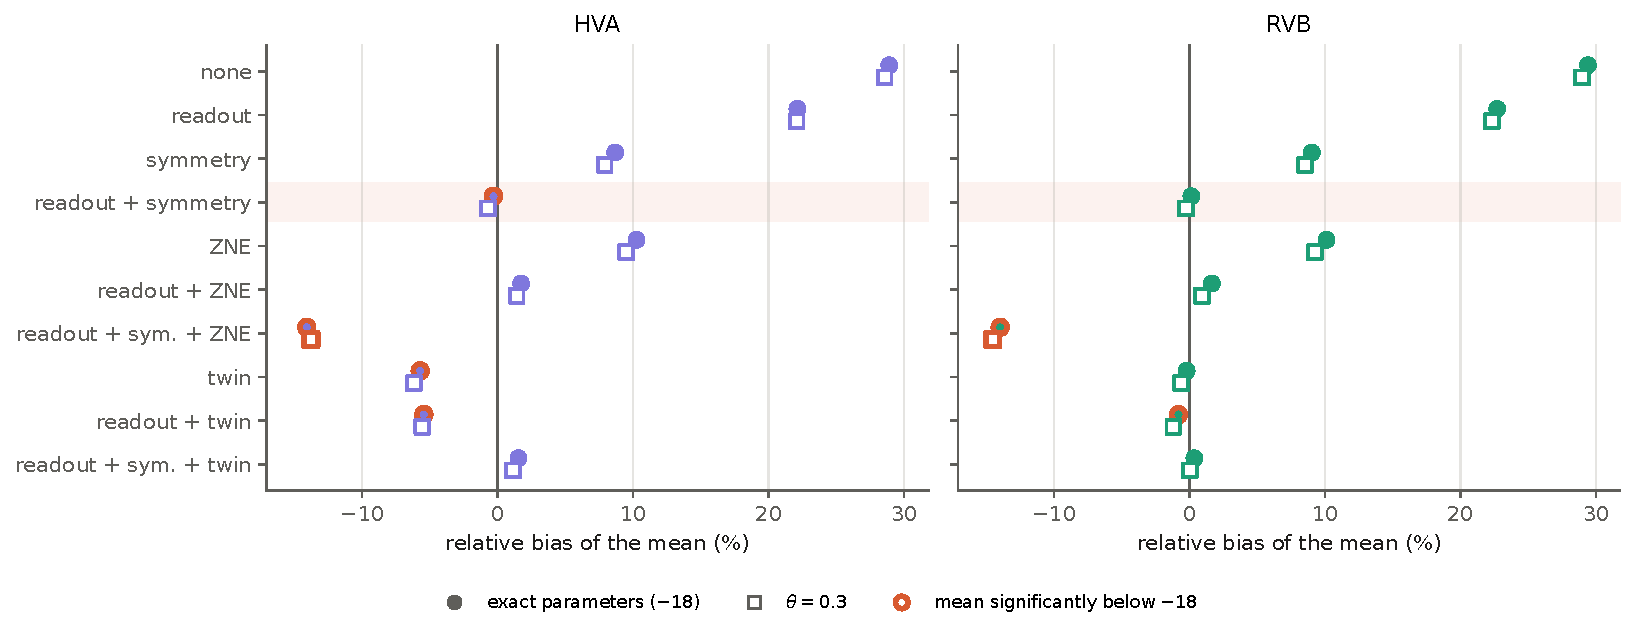
\includegraphics[width=\linewidth]{m2_stacks}
  \caption{The same data as Table~\ref{tab:m2}. Bars: $\pm2$ standard errors of the mean. The
    shaded row is the stack the development session chose. Stacks containing both symmetry and
    ZNE, and the twin stacks for HVA, land far below the noise-free value.}
  \label{fig:m2stacks}
\end{figure}

Figure~\ref{fig:m2stacks} sorts the stacks into three groups.
\begin{itemize}
  \item \textbf{Single techniques remove part of the bias.} Readout correction alone moves HVA at
    $\theta=0$ from \VMtHvaZeroRaw{} to \VMtHvaZeroRo, the readout factor of Table~\ref{tab:floor}.
    Symmetry alone reaches \VMtHvaZeroSym; ZNE alone \VMtHvaZeroZne{} at three times the shots.
  \item \textbf{Two combinations come close.} Readout + symmetry: \VMtHvaZeroRoSymRel{} (HVA) and
    \VMtRvbZeroRoSymRel{} (RVB) at $\theta=0$, \VMtHvaPtRoSymRel{} and \VMtRvbPtRoSymRel{} at
    $\theta=\VBoundTheta$, with no extra shots per energy. Readout + ZNE: \VMtHvaZeroRoZneRel{}
    and \VMtRvbZeroRoZneRel{}, for any ansatz but at three times the shots.
  \item \textbf{Three kinds of stack overshoot.} Symmetry + ZNE goes to \VMtHvaZeroRoSymZne{} (HVA) and \VMtRvbZeroRoSymZne{} (RVB); twin
    rescaling for HVA overshoots by \VMtHvaZeroTwinRel; and readout + symmetry itself is
    \VMtHvaZeroRoSymBelow{} standard errors below $-18$ for HVA at $\theta=0$.
\end{itemize}

\paragraph{Why HVA's twin fails.} HVA's twin is at $(5\pi/4,5\pi/4)$ with noise-free energy
\VMtTwinIdealHva{} and noisy energy \VMtTwinNoisyHva, a rescaling factor \VMtTwinFactorHva. The
target at $\theta=0$ is damped less ($\VMtHvaZeroRaw/{-18}$) than the twin, so the factor
over-corrects. RVB's twin (noise-free \VMtTwinIdealRvb, noisy \VMtTwinNoisyRvb, factor
\VMtTwinFactorRvb) happens to be damped like the target, and rescaling works. The development
session also notes that on the Clifford grid ($\pi/2$ steps) every HVA point is a ground state
or has zero energy, so no Clifford twin exists for HVA on this lattice.

\paragraph{Why symmetry and ZNE do not stack.} The development session's explanation:
post-selection removes noise in a way that is not multiplicative in $\lambda$ (the kept fraction
itself falls with $\lambda$), so the exponential fit extrapolates a curve that does not have the
assumed shape. The observed overshoot, \VMtHvaZeroRoSymZneRel{} at $\theta=0$, is consistent with
that, but this report has not checked the mechanism separately.

\subsection{Why readout plus symmetry looks accurate}
\label{sec:m2cancel}

The development session attributed the small overshoot of readout + symmetry to the calibration
describing all shots while being applied to the post-selected ones. To test that, and to measure
how large the effect is, this report computed the \emph{infinite-shot} value of every
counts-level estimator exactly: the transpiled circuit is simulated as a density matrix, the
outcome distribution of each basis is read without sampling, the device's readout channel is
applied analytically, and the estimators of \cref{dfn:counts} are evaluated on that distribution
(\py{docsgen.physics.mitigation_exact}). The same computation with the full noise model
reproduces the sampled means of Table~\ref{tab:m2} to within their spread (e.g.\ HVA, $\theta=0$:
\VMxHvaZeroFullRaw, \VMxHvaZeroFullRo, \VMxHvaZeroFullSym, \VMxHvaZeroFullRoSym).

\begin{prop}[Filtering then correcting over-corrects]\label{prop:overcorrect}
  Assume independent readout errors with $e_0^{(q)},e_1^{(q)}\le e$, no other noise, and a
  noise-free distribution supported on $|b|=n/2$. Then the filtered distribution is
  $p+O(e^2)$, and to leading order the filter-then-correct estimator returns
  \[
    E_{\mathrm{ro+sym}}=\sum_t c_t\,\langle P_t\rangle\prod_{q\in S_t}\frac{1}{1-e_0^{(q)}-e_1^{(q)}}
      \;+\;O\bigl(e^2,\ \max_q|e_0^{(q)}-e_1^{(q)}|\bigr),
  \]
  a multiplicative over-correction of each two-body term by about $1/(1-2e)^2$.
\end{prop}

\begin{proof}[Proof sketch]
  A single bit flip changes $|b|$ by one, so every read string of weight $n/2$ arises either from
  no flip, with probability $p(b)\prod_q(1-e^{(q)}_{b_q})$, or from at least two flips, with
  probability $O(e^2)$. The kept fraction is $\prod_q(1-e_{b_q}^{(q)})+O(e^2)$, and dividing
  gives $\tilde p=p+O(e^2)$. The filtered shots are therefore already almost free of readout
  error, but the estimator still applies $v_q$. Writing
  $v_q(b)=s(b)/(1-e_0^{(q)}-e_1^{(q)})+(e_0^{(q)}-e_1^{(q)})/(1-e_0^{(q)}-e_1^{(q)})$ and taking
  the product over a two-site support gives
  $\prod_{q\in S_t}s(b_q)\big/\prod_{q\in S_t}(1-e_0^{(q)}-e_1^{(q)})$ up to the stated
  corrections. Averaging over $\tilde p$ gives the formula.
\end{proof}

With the calibrated $e=\VMtReadoutErr$, the predicted factor $1/(1-2e)^2$ is \VMxOverPredicted.
The exact computation with readout noise only gives $E_{\mathrm{ro+sym}}/E_{\mathrm{sym}}=\VMxOverFactor$:
readout + symmetry returns \VMxHvaZeroRoRoSym{} (\VMxHvaZeroRoRoSymRel) at the exact HVA
parameters, where readout correction alone is exact (\VMxHvaZeroRoRo).

\begin{table}[H]
  \centering
  \small
  \begin{adjustbox}{max width=\linewidth}
    % Generated by `uv run python -m docsgen`; do not edit.
\begin{tabular}{lcccc}
\toprule
 & \multicolumn{2}{c}{HVA, $\theta=0$ ($-18$)} & \multicolumn{2}{c}{RVB, $\theta=\VBoundTheta$ (\VMtIdealRvbPt)} \\
\cmidrule(lr){2-3}\cmidrule(lr){4-5}
estimator & readout noise only & full noise & readout noise only & full noise \\
\midrule
none & \VMxHvaZeroRoRaw\,{\small(\VMxHvaZeroRoRawRel)} & \VMxHvaZeroFullRaw\,{\small(\VMxHvaZeroFullRawRel)} & \VMxRvbPtRoRaw\,{\small(\VMxRvbPtRoRawRel)} & \VMxRvbPtFullRaw\,{\small(\VMxRvbPtFullRawRel)} \\
readout & \VMxHvaZeroRoRo\,{\small(\VMxHvaZeroRoRoRel)} & \VMxHvaZeroFullRo\,{\small(\VMxHvaZeroFullRoRel)} & \VMxRvbPtRoRo\,{\small(\VMxRvbPtRoRoRel)} & \VMxRvbPtFullRo\,{\small(\VMxRvbPtFullRoRel)} \\
symmetry & \VMxHvaZeroRoSym\,{\small(\VMxHvaZeroRoSymRel)} & \VMxHvaZeroFullSym\,{\small(\VMxHvaZeroFullSymRel)} & \VMxRvbPtRoSym\,{\small(\VMxRvbPtRoSymRel)} & \VMxRvbPtFullSym\,{\small(\VMxRvbPtFullSymRel)} \\
readout + symmetry (as implemented) & \VMxHvaZeroRoRoSym\,{\small(\VMxHvaZeroRoRoSymRel)} & \VMxHvaZeroFullRoSym\,{\small(\VMxHvaZeroFullRoSymRel)} & \VMxRvbPtRoRoSym\,{\small(\VMxRvbPtRoRoSymRel)} & \VMxRvbPtFullRoSym\,{\small(\VMxRvbPtFullRoSymRel)} \\
correct, then filter (sector-aware) & \VMxHvaZeroRoCtf\,{\small(\VMxHvaZeroRoCtfRel)} & \VMxHvaZeroFullCtf\,{\small(\VMxHvaZeroFullCtfRel)} & \VMxRvbPtRoCtf\,{\small(\VMxRvbPtRoCtfRel)} & \VMxRvbPtFullCtf\,{\small(\VMxRvbPtFullCtfRel)} \\
\midrule
kept fraction (symmetry) & \VMxHvaZeroRoKept & \VMxHvaZeroFullKept & \VMxRvbPtRoKept & \VMxRvbPtFullKept \\
\bottomrule
\end{tabular}

  \end{adjustbox}
  \caption{Infinite-shot energy of each counts-level estimator, with the relative bias in
    brackets. Readout noise only: the device's readout channel and nothing else. Full noise: gate
    errors, $T_1/T_2$ and readout. ``Correct, then filter'' inverts the calibrated readout channel
    on the whole outcome distribution and then projects the resulting quasi-probabilities onto
    weight $n/2$.}
  \label{tab:m2exact}
\end{table}

\begin{figure}[H]
  \centering
  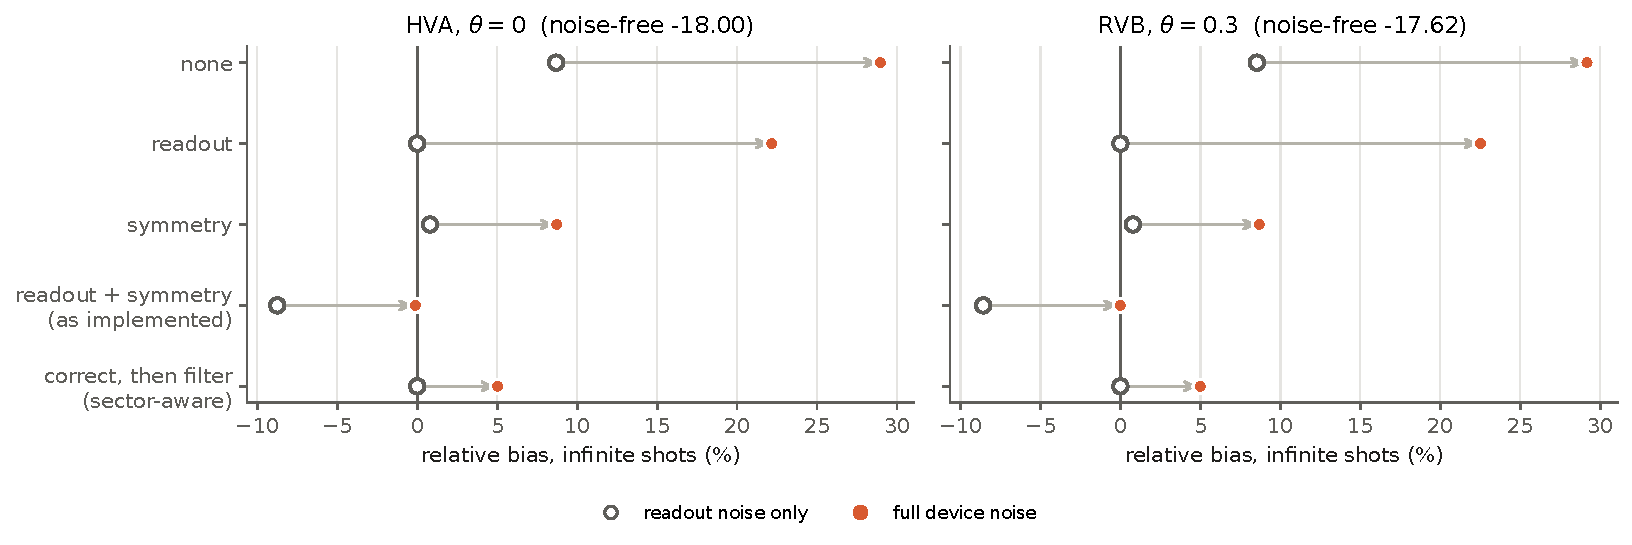
\includegraphics[width=\linewidth]{m2_exact}
  \caption{Each arrow goes from readout noise only (hollow) to full noise (filled). Readout +
    symmetry as implemented starts \emph{below} the noise-free value and is pushed back up by gate
    noise, ending near zero bias by cancellation. Correcting before filtering is exact under
    readout noise and leaves only the gate noise the filter cannot see.}
  \label{fig:m2exact}
\end{figure}

Table~\ref{tab:m2exact} and Figure~\ref{fig:m2exact} separate the two effects.
\begin{enumerate}
  \item \textbf{Readout noise alone} gives readout + symmetry an overshoot of
    \VMxHvaZeroRoRoSymRel{} (HVA, $\theta=0$) and \VMxRvbPtRoRoSymRel{} (RVB,
    $\theta=\VBoundTheta$), as \cref{prop:overcorrect} predicts.
  \item \textbf{Gate noise alone} leaves a bias that symmetry filtering cannot
    remove. The sector-aware estimator, which treats readout consistently, isolates it:
    \VMxHvaZeroFullCtfRel{} and \VMxRvbPtFullCtfRel.
  \item \textbf{Under full noise}, to leading order readout + symmetry equals the symmetry-only
    energy times the over-correction factor: $\VMxOverFactor\times\VMxHvaZeroFullSym=\VMxPredictFull$,
    against \VMxHvaZeroFullRoSym{} computed. The symmetry-only bias (\VMxHvaZeroFullSymRel) and the
    over-correction (\VMxOverPct) happen to be nearly equal on this device.
\end{enumerate}

\begin{rem}[Consequence]
  The small bias of the chosen stack is a property of \py{FakeGuadalupeV2}'s ratio of readout
  error to gate error, not of the method. On a device with relatively less gate noise, or after
  depth compression (M4) removes CX gates, the same stack will move further below the
  noise-free value. Readings below $-18$ in an optimisation are therefore expected, not
  accidental. The sector-aware estimator is principled but leaves \VMxHvaZeroFullCtfRel, and it works with
  quasi-probabilities, so its variance is larger; it was computed here only in the
  infinite-shot limit.
\end{rem}

\paragraph{Follow-up on \py{main}.} The development session reproduced both effects
independently, with sampled runs that switch on one error source at a time. It withdrew the
chosen stack and changed \py{CountsEnergy} to correct then filter when readout and symmetry
are both enabled (commit \texttt{56aadd3}). The new estimator inverts the tensored calibration on
the full $2^n$ outcome distribution and reports a bootstrap standard error, so it is limited to
20 qubits. A new \py{backend.noise} switch (\py{full}, \py{readout}, \py{gates}) makes the
single-source tables part of the benchmark. The reruns (\py{m2b-*}) will decide what to stack on
top of the corrected estimator to remove the remaining gate residual (\VMxHvaZeroFullCtfRel{} at the exact HVA parameters); this
chapter will be updated when they land.

\subsection{Full optimisations with the chosen stack}

\py{configs/m2_mitigated_vqe.toml} reran the M1 recommendations with readout + symmetry
(filter first, as in \texttt{c9272e3}) on the same noise: HVA with plain SPSA (\VMvItersHvaSpsa{} iterations) and RVB with ADAM and parameter
shift (\VMvItersRvbPs{} iterations, \VMvShotsPerRvbPs{} shots per basis).

\begin{table}[H]
  \centering
  \small
  \begin{adjustbox}{max width=\linewidth}
    % Generated by `uv run python -m docsgen`; do not edit.
\begin{tabular}{lcccccc}
\toprule
run & iterations & final energy (re-measured) & rel.\ error & $\sigma$ below $-18$ & noise-free energy of final params & total shots \\
\midrule
HVA, plain SPSA & \VMvItersHvaSpsa & \VMvFinalHvaSpsa ${}\pm{}$ \VMvStdHvaSpsa & \VMvErrHvaSpsa & \VMvBelowHvaSpsa & \VMvIdealHvaSpsa\,{\small(\VMvIdealErrHvaSpsa)} & \VMvShotsHvaSpsa \\
RVB, ADAM + parameter shift & \VMvItersRvbPs & \VMvFinalRvbPs ${}\pm{}$ \VMvStdRvbPs & \VMvErrRvbPs & -- & \VMvIdealRvbPs\,{\small(\VMvIdealErrRvbPs)} & \VMvShotsRvbPs \\
\bottomrule
\end{tabular}

  \end{adjustbox}
  \caption{Mitigated optimisations on \py{FakeGuadalupeV2} noise. The final energy is re-measured
    with 16384 shots per basis through the same stack. The noise-free energy of the final
    parameters (relative error in brackets) is computed classically and measures the
    parameters, independently of the estimator's bias.}
  \label{tab:m2vqe}
\end{table}

\begin{figure}[H]
  \centering
  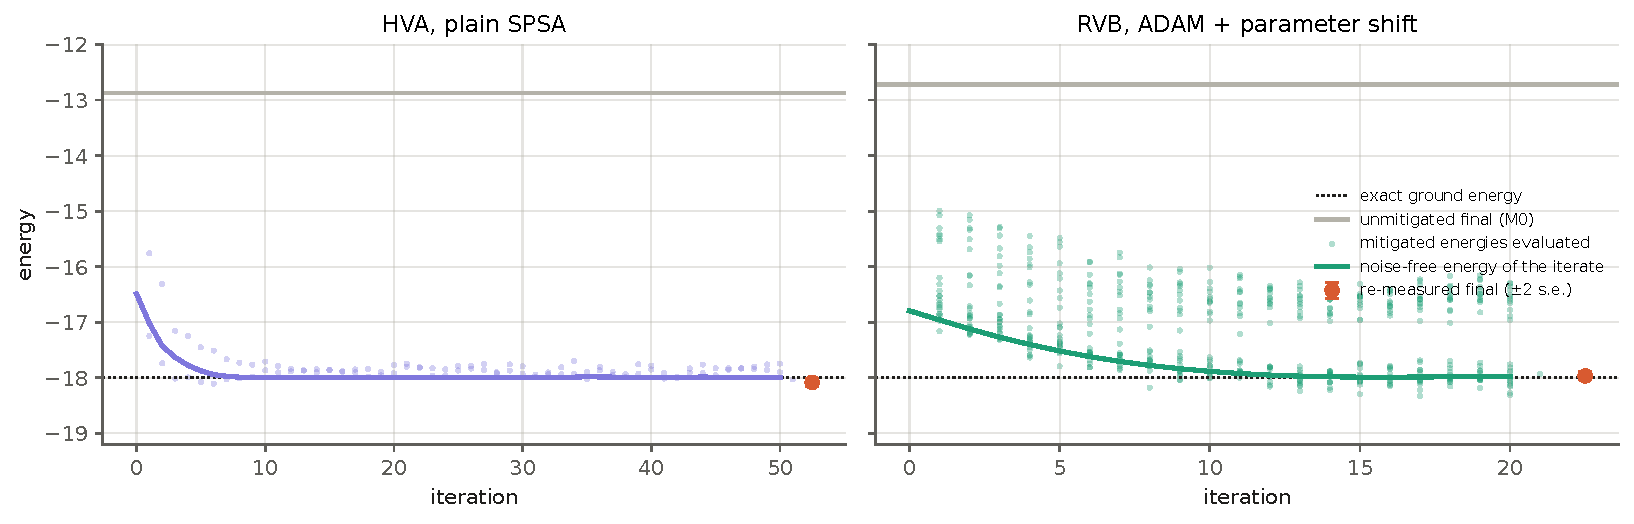
\includegraphics[width=\linewidth]{m2_vqe}
  \caption{Every mitigated energy evaluated (dots), the noise-free energy of the iterate (line),
    and the re-measured final value. Grey: the unmitigated final energy of the same combination
    after M0. ADAM with parameter shift evaluates shifted points, so its dots scatter above the
    iterate.}
  \label{fig:m2vqe}
\end{figure}

Both runs end with parameters whose noise-free energy is within \VMvIdealErrHvaSpsa{} (HVA) and
\VMvIdealErrRvbPs{} (RVB) of $-18$: the optimisers work under mitigation. The re-measured
energies differ from those noise-free values by the stack's bias. HVA reads \VMvFinalHvaSpsa{},
\VMvBelowHvaSpsa{} standard errors below $-18$, which by \cref{prop:mixed} is an artefact. This
is the over-correction of \cref{sec:m2cancel}, not a better state. The total cost is
\VMvShotsHvaSpsa{} and \VMvShotsRvbPs{} shots.

\subsection{Problems solved and open}

\begin{itemize}
  \item[\checkmark] Four mitigation layers, composable, on Aer and the IBM sampler; unit-tested.
    The counts layer reports exact standard errors.
  \item[\checkmark] Fixed-point evaluation mode with a below-ground flag: every stack's bias and
    cost measured at two points.
  \item[\checkmark] Mitigated optimisations reach parameters within \VMvIdealErrRvbPs{} (RVB) and
    \VMvIdealErrHvaSpsa{} (HVA) of the ground energy (noise-free); the estimates read
    \VMvFinalRvbPs{} and \VMvFinalHvaSpsa{} instead of about \VPostFinalRvbAdam.
  \item[$\circ$] \textbf{The chosen stack's accuracy was a cancellation} (\cref{sec:m2cancel});
    the stack is withdrawn. The sector-aware estimator is now on \py{main} (\texttt{56aadd3}).
    Still open: its finite-shot variance, and what removes the remaining gate residual of
    \VMxHvaZeroFullCtfRel{} (reruns pending).
  \item[$\circ$] \textbf{Symmetry and ZNE must not be stacked} as implemented.
  \item[$\circ$] \textbf{HVA has no usable twin}; rescaling is only as good as the twin's damping
    match.
  \item[$\circ$] \textbf{Hardware checks H0 and H1 are skipped}, so neither the noise floor nor
    the mitigation has been tested against a real device.
  \item[$\circ$] \textbf{The instance is easy} (\cref{rem:easy}): at $\theta=0$ the state is a
    singlet product, which symmetry filtering suits unusually well. The generic point confirms
    the trend, but M3 instances are needed before generalising.
\end{itemize}

\subsection*{Exercises}

\begin{exer}
  A qubit has $e_0=0.02$ and $e_1=0.03$. Compute $v(0)$ and $v(1)$, and check
  $\mathbb E[v(\tilde b)\mid b=1]=-1$.
\end{exer}
\begin{sol}
  $1-e_0-e_1=0.95$, so $v(0)=(1-0.03+0.02)/0.95=0.99/0.95\approx1.0421$ and
  $v(1)=-(1+0.03-0.02)/0.95=-1.01/0.95\approx-1.0632$. Given $b=1$, the read bit is $0$ with
  probability $e_1=0.03$, so the mean is $0.03\cdot1.0421+0.97\cdot(-1.0632)=0.03126-1.03126=-1.0000$.
\end{sol}

\begin{exer}
  Under readout noise only, why is symmetry filtering by itself \emph{not} exact
  (Table~\ref{tab:m2exact}: \VMxHvaZeroRoSymRel), although it removes every single-flip error?
\end{exer}
\begin{sol}
  Two flips in opposite directions ($0\to1$ on one qubit and $1\to0$ on another) keep the weight
  at $n/2$ and pass the filter. They occur with probability $O(e^2)$ per shot, but there are
  many qubit pairs: about $\binom{12}{2}\,e^2\approx66\times(0.022)^2\approx3\,\%$ of shots carry
  a double flip, a fraction of which pass. A pair flip inside a bond changes that bond's $Z_iZ_j$
  reading only if exactly one of its qubits flips, which biases the energy upward by a fraction
  of a percent.
\end{sol}

\begin{exer}
  Using the twin data of the HVA row, predict the twin-rescaled energy at $\theta=0$ from the raw
  mean, and compare with Table~\ref{tab:m2}.
\end{exer}
\begin{sol}
  $E_{\mathrm{mit}}=\VMtHvaZeroRaw\times\VMtTwinIdealHva/\VMtTwinNoisyHva=\VMtHvaZeroRaw\times\VMtTwinFactorHva\approx-19.0$,
  matching the twin row, \VMtHvaZeroTwin. The raw estimate and the twin come from separate runs,
  so the agreement is within the spread. The overshoot follows from the target being damped by
  $12.80/18\approx0.711$ and the twin by $7.56/11.25\approx0.672$.
\end{sol}
